
Originally our focus was on reproducing graph based security metrics. While we have since expanded the scope to include the range of metrics that can be applied to any area of cyber security, the metrics which exploit the relationships between components in the system typically require the most preprocessing to shape the inputs correctly. For instance, a count of the number of critical vulnerabilities found from a scan is a straight forward metric calculation. Determining which vulnerabilities are reachable in a given network topology requires more effort, and ensuring that reachability graph conforms to the assumptions of the target metric (non-invertable weighted transition matrix or some other specific representation) requires still further computation. Thus, PTaH exposes some general statistical methods for the simpler metrics as well as some more fine grained helpers that apply to subsets or individual metric implementations. In this way we can maintain the simple abstractions of both the raw input source and the actual metric calculation, while also supporting the preprocessing requirements for new metrics. As mentioned above, there are many ETL pipeline implementations available which would be suitable for this implementation, so in this section we demonstrate examples of metric specific data transformations rather than the underlying technology used to execute them. 

The attack graph models described in the literature vary somewhat in structure among implementations. For example, the AGs presented in \cite{Ou_Appel_2005} include non-exploits along with exploits as nodes with edges representing lateral movements. In \cite{Noel_Jajodia_2014} the non-exploit nodes don't appear to be present in the publication, although the TVA tool isn't publicly available to test this. In \cite{Dacier_1994} and \cite{Ortalo_1999} nodes represent system privileges and edges contain exploits that grant an attacker additional privileges on a set of systems, while in \cite{Phillips_Swiler_1998} edges carry probabilities of exploitation and the nodes represent actual hosts. While the differences are subtle, they do require an understanding of the target input expected by each metric. In these cases, our solution is to provide helper methods that transform the provided knowledge base into any of these expected input formats. If an attack graph is needed for processing, relevant system information is translated into datalog facts for use in MulVal\cite{Ou_Appel_2005}. MulVal consists of 2 primary components, an XSB Datalog program that computes attack traces from a given set of facts and interaction rules, and a C++ program that processes the XSB output trace and produces an annotated list of vertices and edges corresponding to possible attack paths. To allow more control over MulVal processing we replaced the driver shell script with a python interface, allowing programmatic access to the facts and interaction rules that are used to derive attack graphs directly over a Python-XSB bridge. This allows us to manipulate structural properties of the input system and delegate vulnerability placement strategically while avoiding many of the high cost disk operations that the original controller required. 



While the differences are subtle, they are enough to necessitate a general form of attack graph which we present in Figure \ref{fig:automation:ag_uml}. Our representation of an attack graph is a multi-edged directed acyclic graph.     

% % \begin{wrapfigure}[10]{I}{.25\textwidth}
% \begin{figure}[H]
% \centering
% 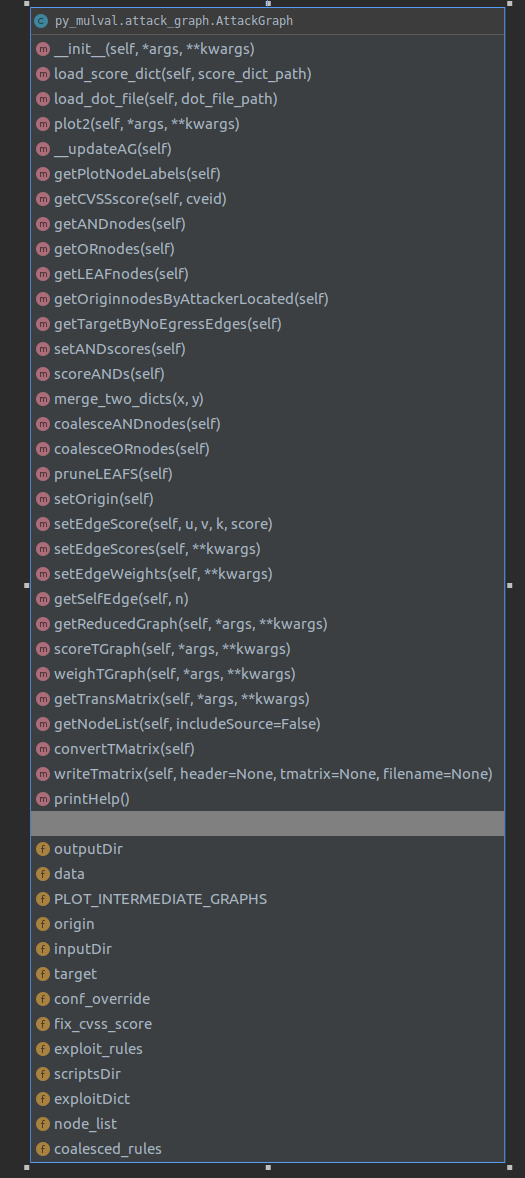
\includegraphics[scale=.45]{resource/img/ch_automation/attack_graph_class_diag.png}
% % \end{wrapfigure}
% \caption{Attack Graph Methods and Properties}
% \label{fig:automation:ag_details_uml}
% \end{figure}

% As shown in Figure \ref{fig:automation:ag_details_uml}, our implementation allows us to load various AG formats from graph description language (.dot) files, from adjacency lists as shown in Tables \ref{tab:eg_verts} and \ref{tab:eg_arcs}, or other formats as specified. Once loaded, we provide programmatic access to manipulate scoring and weighting functions, exploits definitions, and vulnerability scores. This allows for a simple means to test the range of values a metric will generate, the sensitivity of a metric to fluctuations in parameters, and how well a metric performs on different models. It also gives us some insights into how well each AG type actually models threat and defense attributes.

In Figure \ref{fig:transGraph}, we show the process of ingesting an attack graph produced by MulVal\cite{Ou_Appel_2005} and transforming it into a normalized weighted graph for export to a dense transition matrix used in several probabilistic security metrics. A MulVal attack graph contains three types of nodes. Referring to Figure \ref{fig:tg_001},  \textit{LEAF} nodes (green rectangles) describe known facts like configuration information and attacker privilege that are given as inputs to the system model. Internal nodes generally represent potential privileges to be gained by an attacker.  \textit{AND} nodes (red ovals) contain interaction rules that dictate which facts and conditions are necessary to derive new knowledge. \textit{OR} nodes (blue diamonds) represent derived facts such as transition states possible given all incoming conditions are satisfied. Each step in the reduction process can be called explicitly via API to produce the desired result, or the composition of a series of individual transforms can be exposed as a single call.  

Once loaded, we provide programmatic access to manipulate scoring and weighting functions, exploit definitions, and vulnerability assignments. This allows for a simple means to test the range of values a metric will generate, the sensitivity of a metric to fluctuations in parameters, and how well a metric performs on different models. It also gives us some insights into how well each AG type actually models threat and defense attributes. While we focus on attack graphs in this paper, the process for manipulating other threat model structures (such as attack trees or nets) is similar, where the goal is to introduce controlled perturbations in the representation without altering its fundamental structure to assess the behaviour of the target metric.

% \begin{minipage}{.95\linewidth}
\begin{lstlisting}[language=yaml, label={lst:coalesce}, caption={Node Labels to Coalesce},captionpos=b, ]]
coalesce_rules: # list of AND rules to coalesce
  - 'multi-hop access by gateway'
  - 'multi-hop access'
  - 'direct on-host access'
  - 'direct network access'
  - 'log in for ftpd'
  - 'Access a host through a log-in service'
  \end{lstlisting}
% \end{minipage}

The dictionaries shown in Listings \ref{lst:coalesce}, \ref{lst:exploit}, and \ref{lst:exploit_dict} provide granular control over the transformation process and can be defined statically at compile time via yaml syntax (shown), or generated dynamically at runtime and set as properties of the associated object being transformed. 

The coalesce rules shown in Listing \ref{lst:coalesce} define which types of transitions should be ignored in the final result. If we consider an adjacency matrix $M$ where the connections between two vertices represent the likelihood of successful exploit, then in cases where no exploit was used, how is the transition represented? Leaving the value at zero may result in a non-invertable or improperly weighted result, so we simply merge any transitional edges that occur as a result of one of the rules in this dictionary.

% \begin{minipage}{.94\linewidth}
\begin{lstlisting}[language=yaml, label={lst:exploit}, caption={Fixed Scores for Exploit Classes},captionpos=b, ]]
exploit_rules: # dict of AND rules to add to tmatrix
  'remote exploit of a server program': 3
  'Trojan horse installation': 4
  'local exploit': 5
  'NFS shell': 7
  'execCode implies file access': 8
  'NFS semantics': 9
  'any machine he has an account on will also be compromised': 9.2
  'through a log-in service': 9.3
  'password sniffing through spoof': 4
  'password sniffing through route hijack': 5.6
\end{lstlisting}
% \end{minipage}

Similar in behavior to the coalescing rules above, we can also fix transition scores of classes of transitions based on the interaction rule they fire. This allows us to test the effects of changing the exploitability or impact scores on classes of vulnerabilities based on the outcome of that successful exploit without needing to identify every possible vulnerability that produces that outcome.

% \begin{minipage}{.95\linewidth}
\begin{lstlisting}[language=yaml, label={lst:exploit_dict}, caption={Override Specific Vulnerability Scores},captionpos=b,]]
exploitDict: # dict of LEAF CVSS overrides
  'CVE-2014-9796': 6.1
  'CVE-2009-2048': 6.2
  'CVE-2015-7501': 6.3
  'CVE-2016-xxxx': 1.4
  'CAN-2002-0392': 6.5
  'CVE-2010-2784': 6.6 # no sql cnxn
  'CVE-2014-6271': 6.7
  'arpSpoofVuln': 6.8
  'vulID': 6
\end{lstlisting}
% \end{minipage}

Listing \ref{lst:exploit_dict} allows us to fix any specific vulnerability score individually. The override precedence favours specific over general, so individual scores set here will be applied after scoring based on exploit rules and globally fixing scores. Finally, a default scoring strategy which supports dataset queries such as NVD, or returning a fixed weight if preferred.

% \begin{minipage}{.95\linewidth}
\begin{lstlisting}[language=Python, label={lst:map_mttf}, caption={Map CVSS to MTTF},captionpos=b,]]
# from Dacier_1996
# .0002 is quasi-instantanious
# .02 is 1 hour
# .2 1 day
# 1 is 1 week
# 5 is one month
# 50 is one year
# we invert so scores reflect 
# mean transition rates (lambda)
time_dict = {(0, 1.6): 1. / .0002,
             (1.6, 3.3): 1. / .02,
             ( 3.3, 5): 1. / .2,
             (5, 6.6): 1. / 1.,
             (6.6, 8.3): 1. / 5.,
             (8.3, 10): 1. / 50., }
\end{lstlisting}
% \end{minipage}

As shown in Figures \ref{fig:gm_002} and \ref{fig:gm_001}, we can also map scored graphs between systems. Listing \ref{lst:map_mttf} demonstrates how we can map an interval, in this case CVSS score ranges, to a fixed value like the MTTF arrival rates provided by Dacier\cite{Dacier_Deswarte_Kaaniche_1996a}. In Figure \ref{fig:gm_003} we apply a globally fixed CVSS score to the graph which preserves the MTTF mapping, and subsequently remove the mapping in Figure \ref{fig:gm_004} to return to the CVSS scoring strategy. By instrumenting the transformation pipeline to support fine grained variations of the structures and values passed to security metrics, we can study how these metrics perform in a variety of scenarios, validate the metrics against a set of functional criteria, and select appropriate security metrics based on performance against a desired reference set.
